\section*{Points de départ}
\subsection*{RDF}
\paragraph{}
RDF est l’abréviation de “Resource Description Framework” qui se base sur un modèle de graphe. Il s’agit d’un cadre de description de ressources, d’une façon formelle sur le web.
C’est la première brique de standard du web sémantique qui recouvre à la fois un modèle et plusieurs syntaxe pour publier des données variées sur le web.
\subparagraph{}
Dans RDF ~: 
\newline 
\begin{itemize}
\item Les ressources sont un concept de base du web sémantique. D’où:  “tout ce qui peut être référencé est une ressource”. Et dans un contexte plus technique: On déduit que tout ce qui peut être identifié par un URI/IRI peut être considéré comme ressource.
\item  Un ensemble d’attributs décrivent la ressource, qui possèdent des caractéristiques et des relations avec d’autres ressources.
\item Le cadre standardise la syntaxe de ces descriptions, les modèles et les langages.  
\end{itemize}
\subparagraph{}
La plus petite structure de description en RDF est le triplet (fig).
\begin{figure}[H]
        \centering
                \centering
                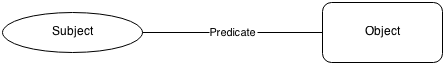
\includegraphics[width=10cm]{tripletrdf.png}
               \caption{triplet RDF}

\end{figure}
\subparagraph{}
Un triplet décrit une ressource, l’associe à une propriété et une valeur de cette propriété qui peut être une nouvelle ressource liée. Par exemple “Moncef a écrit une page QuadsRDF.html à propos des quadruplets RDF” peut être décomposée en deux triplets ayant comme sujet “QuadsRDF.html”:
<QuadsRDF.html, auteur, Moncef>(figure2) et <QuadsRDF.html, thème, quadruplets RDF>(figure3).
On peut schématiser cela de la manière suivante:
\begin{figure}[H]
        \centering
                \centering
                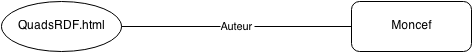
\includegraphics[width=10cm]{moncef.png}
               \caption{Exemple 1}

\end{figure}
\begin{figure}[H]
        \centering
                \centering
                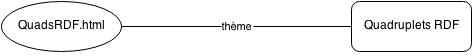
\includegraphics[width=10cm]{quads.png}
               \caption{Exemple2}

\end{figure}
\subsection*{DBpedia}
\paragraph{}
C'est un projet universitaire et communautaire d’extraction et d’exploitation automatique des données de wikipedia. C’est un ensemble de données structurées et normalisées au format du web sémantique.
DBpedia 3.9 est la dernière version de DBpedia datant de Juin 2013. DBpedia est écrite en Scala et Java.
Elle adopte les normes du web sémantique et du réseau Linked Open Data. Pour chaque document encyclopédique, il existe une page de ressources contenant toutes les données sous forme de triplets RDF.
\begin{figure}[H]
        \centering
                \centering
                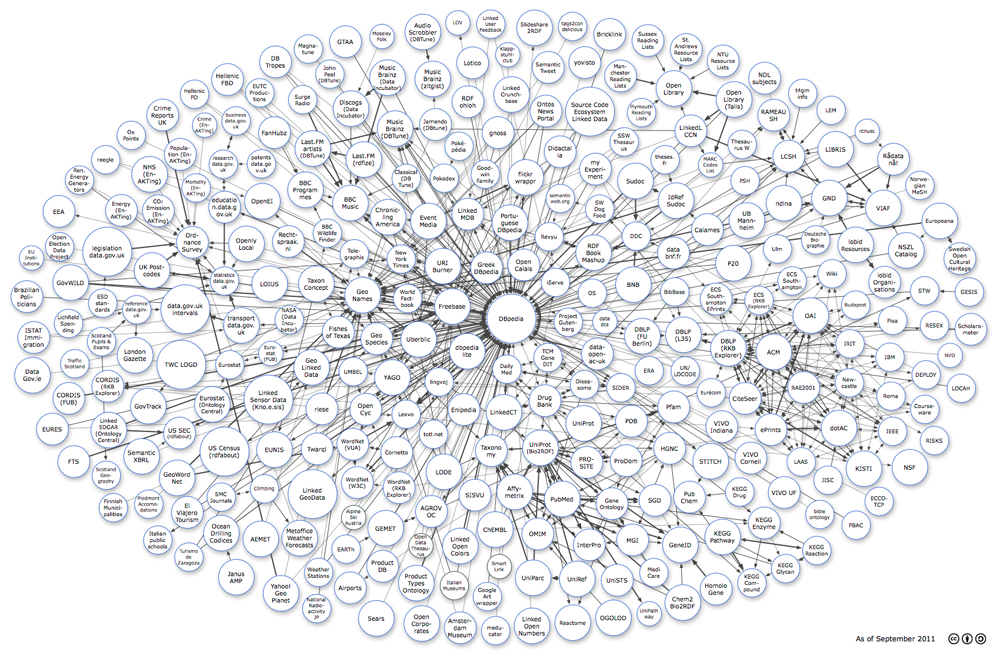
\includegraphics[width=10cm]{dbpedia.png}
               \caption{DBpedia}

\end{figure}
\newpage
\section*{Proposition}
\subsection*{Problématique}
\paragraph{}
Lorsqu’on parcours un document “Wikipedia” on trouve beaucoup d’informations temporelles qui sont généralement liées à un contexte précis.
Il est plus difficile d’exploiter ces informations si elles ne possèdent pas une structure claire et lisible par la machine.
\newline
Il se trouve que des informations temporelles dans DBpedia sont exprimées de la manière suivante: 
\begin{figure}[H]
        \centering
                \centering
                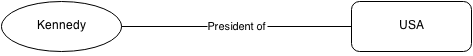
\includegraphics[width=10cm]{ken.png}
               \caption{triplet ''Kennedy''}

\end{figure}
\subparagraph{}
Il est toujours possible d’exprimer le temps dans sous forme de un triplet comme l’exemple ci-dessous: 
\begin{figure}[H]
        \centering
                \centering
                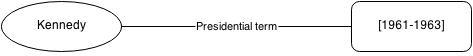
\includegraphics[width=10cm]{presidterm.png}
               \caption{triplet presidential term ''Kennedy''}

\end{figure}
\subparagraph{}
Dans notre sujet de recherche on vise plutôt à annoter les triplets (s,p,o) avec une étiquette temporelle qui précise la validité de ce terme dans un cadre logique qui appartient au monde réel où en dehors de ce cadre, on peut dire que ce triplet RDF n’est pas valide et qu’on ne peut pas l’utiliser.
\subsection*{Sources de données}
\paragraph{}
Les données brutes proviennent de sources distinctes~:
\subsubsection*{Texte Wikipedia}
\paragraph{}
On cherche à extraire les informations temporelles qui ont un contexte de validité lié à un fait à partir des données textuelles des pages de Wikipedia. 
Par exemple sur la page de John Fitzgerald Kennedy, on retrouve~:
\newline
Kennedy a visité Berlin Ouest le 23 Juin 1963.
\subparagraph{}
On veut extraire les ressources en donnant une nouvelle structure pour mieux présenter leur contexte de validité temporelle.
\subsubsection*{Info box Wikipedia}
\paragraph{}
On remarque sur la section droite de la page wikipedia des informations temporelles plus structurées indiquant généralement des intervalles de temps pour des évènements importants sur la personne ou le sujet de la page (fig):
\begin{figure}[H]
        \centering
                \centering
                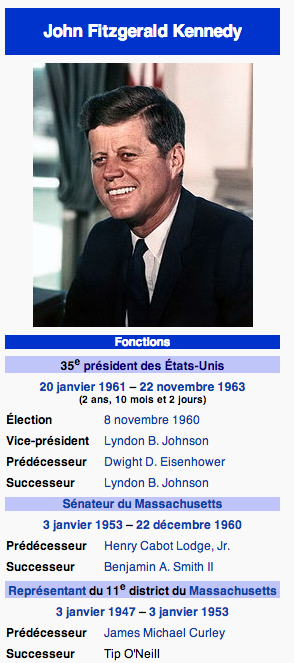
\includegraphics[width=5cm]{kennedy.png}
               \caption{Info Box Wikipedia ''Kennedy''}

\end{figure}
\subsubsection*{Tableau}
\paragraph{}
Dans les tableaux “Wikipedia” figurent des informations temporelles plus structurées et plus faciles à extraire, qu’on cherche à récupérer.
\subparagraph{}
Vous trouverez ci-dessous des informations sur les anciens précidents des États-Unis.
\begin{figure}[H]
        \centering
                \centering
                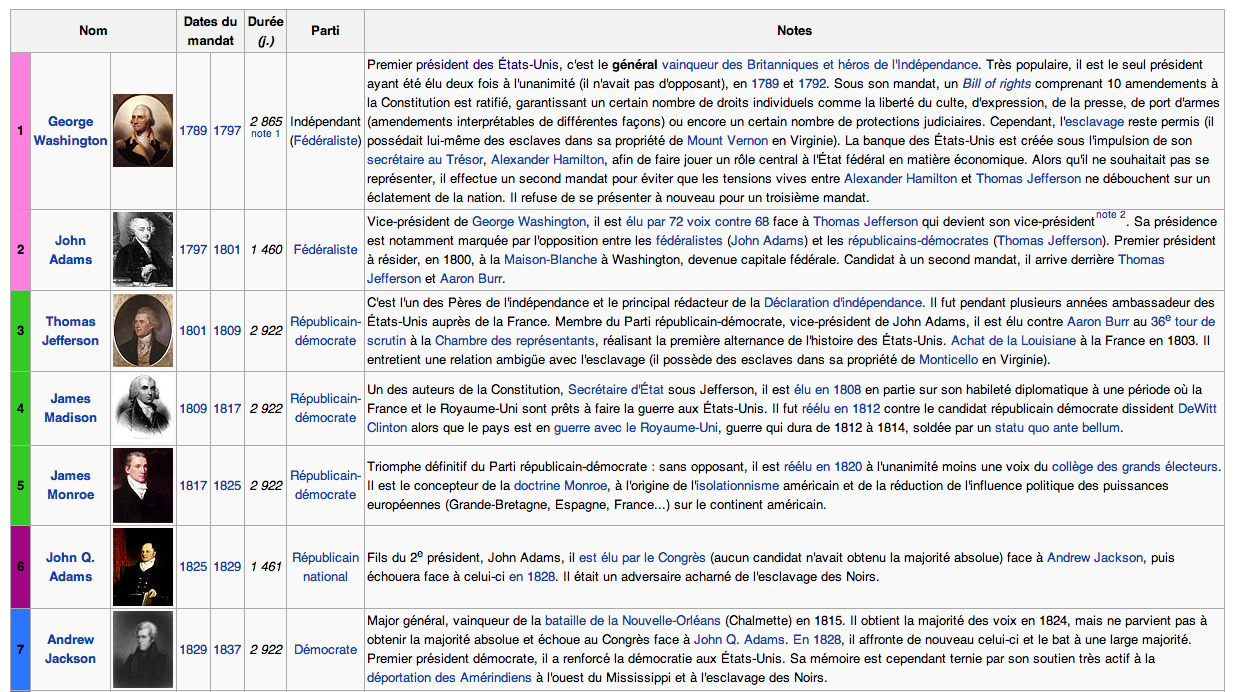
\includegraphics[width=14cm]{tableau.png}
               \caption{Exemple de tableau Wikipedia}

\end{figure}
\subsubsection*{Wikidata}
\paragraph{}
Sur la page wikidata, liée au contenu de la page wikipedia de Kennedy, on a intérêt à extraire les informations temporelles (fig).
\begin{figure}[H]
        \centering
                \centering
                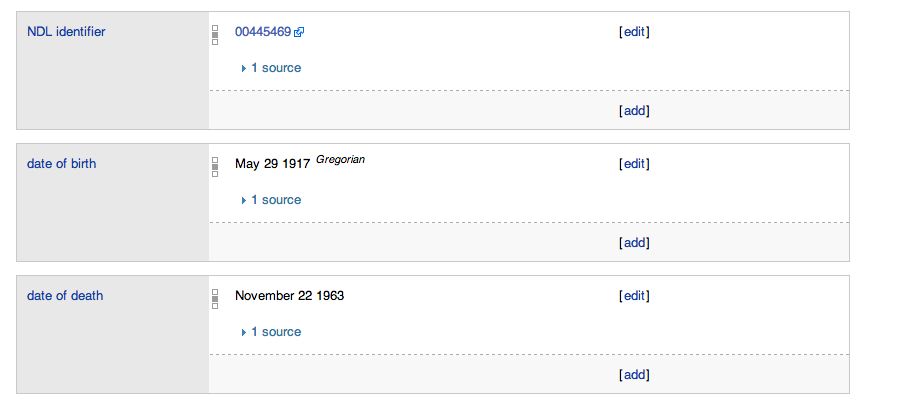
\includegraphics[width=14cm]{wikidata.png}
               \caption{Exemple Wikidata}

\end{figure}
\subsubsection*{Historique des pages wikipedia}
\paragraph{}
On souhaite, si c’est possible, extraire des informations temporelles relatives à l’historique de modifications des pages de wikipedia. Car, il se trouve qu’il y on a beaucoup d’informations liées à cet historique.
\subsubsection*{Résumé}
\paragraph{}
Il s'avère que beaucoup de points du temps dont liées à plusieurs sources d’information évènementielle; on cherche à extraire ces informations afin de les mettre sous une forme plus adéquate.
\subsection*{Notre modélisation}
\paragraph{}
Pour surmonter ce problème et exprimer la validité temporelle d’un triplet RDF d’une manière à la fois intelligente et lisible par la machine; on souhaite rattacher au triplets valides que dans une plage temporelle bien précise une étiquette temporelle adéquate.
\newline
Exemple~:
\begin{figure}[H]
        \centering
                \centering
                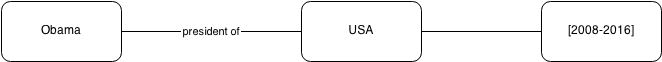
\includegraphics[width=10cm]{obamaQuad.png}
               \caption{Modélisation quadruplet}

\end{figure}
\subparagraph{}
On s'intéresse au format N-Quads qui est un standard w3c basé sur la forme N-Triples. L’avantage est qu’il se distingue par la possibilité d’encoder des graphes multiples.
Les quadruplets vont être formalisés de la manière suivante~:
\newline
$<s,p,o,[t1,t2]>$, un sujet, prédicat, objet avec une intervalle de temps.
\newline
$<s,p,o,t>$, de même avec un point de temps $t$.
\subsubsection*{Schéma de modélisation}
\paragraph{}
Tout d’abord, et à partir des différents sources d’informations on veut récupérer les informations temporelles dans leurs contextes sémantiques à l’aide de nos différents extracteurs implémentés. 
Ensuite, les mettre dans un ensemble de fichiers comme le montre le schéma ci-dessous.
Enfin, on essaye de proposer cette nouvelle structure à l’équipe DBpedia.
\begin{figure}[H]
        \centering
                \centering
                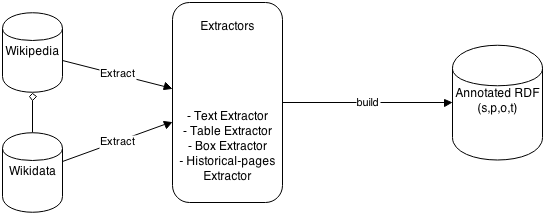
\includegraphics[width=10cm]{modelisation.png}
               \caption{Modélisation générale}

\end{figure}
\section*{Analyse temporelle}
\subsection*{Représentation}
\paragraph{}
Les informations temporelles peuvent avoir des repèsentations différentes~: 
\begin{itemize}
\item D'un évènement `` Je vous propose un rendez-vous $demain$ pour parler de mon projet 'WeShare' ``. \item D'une connaissance `` Jacques Chirac est le président de la république Française `` \textbf{ mais quand ?}.

\end{itemize}
 
\subsection*{Ambiguïtés temporelles}
Le présent par exemple peut avoir plusieurs sens ou contextes : présent de narration, présent de généralité, présent qui réfère au futur proche, etc...
\subparagraph{}
Les signaux temporelles sont ambigus~: réunion de 14h à 16h, il court pour rattraper le temps, tu tournes après la rivière, etc…
\subparagraph{}
La plupart des expressions sont floues~: il y a deux ans, chaque deux semaines, j’arrive dans deux secondes, etc...
\paragraph{}
L’analyse du temps s’inscrit dans la compréhension globale des textes, et des évènements auxquels on fait référence dans ce texte. 
\newline
Modalité~: l’équipe de France voulait gagner la coupe du monde en 2006. 
\newline
Anaphore~: cela pourrait avoir lieu dans les éditions suivantes.
\subparagraph{}
Les évènements décrits (et que l’on souhaite fixer temporellement) peuvent être: duratifs ou ponctuels/accomplis ou inaccomplis. 
\subparagraph{}
De même pour les dates qui peuvent être~: Date absolue ``18 mars 1990 c'est mon anniversaire``; Date relative par rapport au moment de l’énonciation~: `` il y a deux ans ``. Pour la durée~: Durée absolue `` durant 2 ans ``; Durée relative~: `` depuis un an ``.
\subparagraph{}
On trouve aussi~: Expression de fréquence `` tous les ans, le vendredi 13 ``, Expression plus complexe `` après la Révolution Tunisienne ``.
\subsection*{Résumé}
\paragraph{}
Dans un texte simple il se trouve qu’on a beaucoup d’informations temporelles. On s'intéresse aussi au sémantique du contenu bien évidement. Dans ce travail on va plutôt essayer d’extraire les dates saillantes.








